% Chapter Title Page
\clearpage
\thispagestyle{empty} 
\begin{center}
    \vspace*{\fill} 
    \Huge \textbf{Chapter 7} \\
    \Huge \textbf{Cryptographic Hash Functions} 
    \vspace*{\fill}
\end{center}
\clearpage

\chapter{Cryptographic Hash Functions}

\section{Definition}
A hash function takes an input of arbitrary length and maps it to a fixed-length data block. Multiple input blocks may produce the same output, known as the hash value or hash digest.

\section{Requirements for Cryptographic Hash Function}

\begin{table}[h!]
\centering
\begin{tabular}{|p{3.5cm}|p{9cm}|}
\hline
\textbf{Requirement} & \textbf{Description} \\
\hline
Variable input size & Can be applied to a block of data of any size. \\
\hline
Fixed output size & Produces a fixed-length output. \\
\hline
Efficiency & Relatively easy to compute for any given input, making hardware and software implementations practical. \\
\hline
Preimage resistant & Computationally infeasible to find an input that maps to a given hash value. \\
\hline
Second preimage resistant & Computationally infeasible to find a different input with the same hash value. \\
\hline
Collision resistant & Computationally infeasible to find any two different inputs that map to the same hash value. \\
\hline
Pseudorandomness & Output appears to be a random sequence of bits. \\
\hline
\end{tabular}
\caption{Requirements for Cryptographic Hash Function}
\end{table}
\begin{figure}
    \centering
    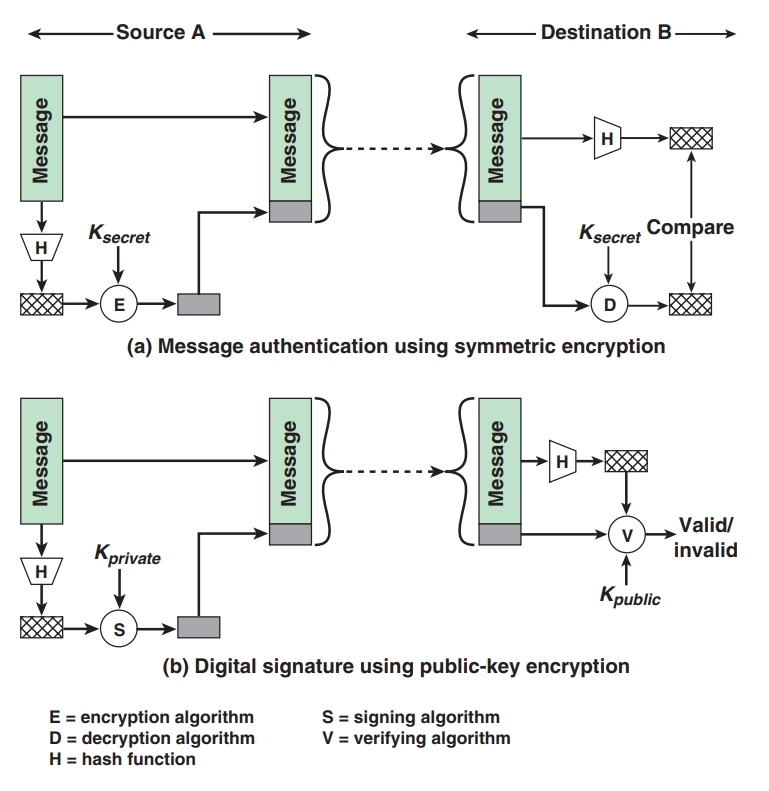
\includegraphics[width=1\linewidth]{Data_Privacy_and_Cryptography/Figures/use of secure hash fun.jpeg}
    \caption{Uses for a Secure Hash Function}
    \label{fig:hashfunction}
\end{figure}


\section{Uses of Cryptographic Hash Functions}

\subsection{Message Authentication:}
Ensures data integrity and verifies the authenticity of the message source. 

Example process:
\begin{enumerate}
    \item Generate a hash value for the source message.
    \item Encrypt the hash value using a secret key shared by a cooperating partner.
    \item Transmit the message plus the encrypted hash value to the destination.
    \item The recipient decrypts the hash value, generates a new hash value from the incoming message, and compares the two hash values.
\end{enumerate}

\subsection{Digital Signatures:}
Verifies the origin and integrity of a message. The sender's private key is used to encrypt the hash value, and the recipient can use the sender's public key to decrypt it and verify the message.

\section{Digital Signatures}

\subsection{Definition:}
A cryptographic transformation of data ensuring origin authentication, data integrity, and non-repudiation (NIST FIPS 186-4).

\subsection{Process:}
\begin{enumerate}
    \item \textbf{Hash Generation:} Bob generates a hash value for his message using a secure hash function.
    \item \textbf{Signature Creation:} Bob uses his private key and the hash value to create a digital signature.
    \item \textbf{Sending:} The message is sent with the digital signature attached.
    \item \textbf{Verification:} \begin{enumerate}
    \item The receiver generates a hash value of the received message.
    \item The receiver uses Bob’s public key, the generated hash, and the received signature to verify the message.
    \item If valid, it confirms the message was indeed sent by Bob and hasn’t been altered.
\end{enumerate}
\end{enumerate}


\subsection{Applications:}
\begin{itemize}
    \item Signing email messages for sender authentication.
    \item Signing software programs to authenticate their source and counter software tampering.
    \item Verifying authorship or origin of digital data.
    \item Ensuring the integrity of digital data against tampering.
    \item Authenticating online entities.
\end{itemize}

